\documentclass{article}

% Language setting
% Replace `english' with e.g. `spanish' to change the document language
\usepackage[english]{babel}
\usepackage{float}

% Set page size and margins
% Replace `letterpaper' with `a4paper' for UK/EU standard size
\usepackage[letterpaper,top=2cm,bottom=2cm,left=3cm,right=3cm,marginparwidth=1.75cm]{geometry}

% Useful packages
\usepackage{amsmath}
\usepackage{graphicx}
\usepackage{caption}
\usepackage[colorlinks=true, allcolors=blue]{hyperref}

\usepackage{titling}

\setlength{\droptitle}{-1cm}    % Moves the title *up* (adjust as needed)
\pretitle{\vspace{-1cm}\begin{center}\Huge\bfseries}
\posttitle{\end{center}\vspace{-0.5cm}}  % Space *after* title

\title{Encounters of the Fibrous Kind}
\author{Clint Wang, Jeffery Xu}

\begin{document}
\maketitle

\section{Introduction and Theory}

We built a real-time physical simulation framework for rigid and fabric-like objects using extended position-based dynamics (XPBD) \cite{Macklin:2016:XPS:2994258.2994272}. To evaluate the strengths and limitations of XPBD, we extended a baseline shape-matching PBD cloth simulation with self-collision handling, friction constraints, and collisions against rigid bodies. After discovering the limitations of shape-matching and triangular meshes, we implemented a particle cloth that uses distance constraints. We then created a real-time origami simulation by adding stiff hinge constraints to the cloth model. 

\subsection{Extended Position-based Dynamics}
The baseline cloth simulation uses position-based dynamics (PBD), which can be thought of as a Verlet-like position prediction step, followed by an implicit-style constraint projection. The constraint solver computes a per-constraint position delta:
\[\Delta x = k_js_j\textbf{M}^{-1}\nabla C_j(\textbf{x}_i)\]
The subscript $i$ denotes the iteration index, $j$ denotes the constraint index, $k_j \in [0, 1]$ is the constraint stiffness, $C$ denotes the constraint function, and the scaling factor $s_j$ is derived:
\[s_j = \frac{-C_j(\textbf{x}_i)}{\nabla C_j\textbf{M}^{-1}\nabla C_j^T}\]
The issue with PBD is that stiffness depends on the number of constraint projections performed. XPBD solves this by introducing compliance $\alpha$ (block diagonal compliance matrix corresponding to inverse-stiffness) and a Lagrange multiplier per constraint:
\[\Delta \textbf{x} = \textbf{M}^{-1}\nabla \textbf{C}(\textbf{x}_i)^T \Delta \lambda\]
XPBD solves $\Delta \lambda $ by approximating each constraint as a local linear system and performing a Gauss-Seidel update:
\[\Delta \lambda = \frac{-C_j(\textbf{x}_i)-\tilde\alpha_j\lambda_{ij}}{\nabla C_j \textbf{M}^{-1}\nabla C_j^T + \tilde\alpha_j}\]
XPBD folds the time step into compliance, defining $\tilde\alpha = \frac{\alpha}{\Delta t^2}$. Because shape-matching does not easily provide a scalar $C$, we chose to keep shape-matching in PBD while creating a new distance constraint option in XPBD:
\[C(\textbf{x}) = |\textbf{x}_i - \textbf{x}_j| - L_0\]
Users can toggle between the two. 

\subsection{Self-Collision and Rigid Bodies}
For both the triangle and particle cloth collision-detection, we used a spatial hash. The triangle cloth hashes triangles and runs vertex-triangle continuous collision detection (CCD). The particle cloth hashes particles and runs vertex-vertex and sub-stepping. 

Our implementation of continuous-collision detection predicts collisions along a path by solving for the earliest exact $t$ in $\hat x = x+dx\Delta t$ where $\hat x$ intersects any object. We discovered that CCD with triangles is computationally expensive and assumes linear approximation of motion resulting in tunneling. 

To solve this, we implemented a particle cloth simulation where collisions are tested between vertex particles with a set radius. Since XPBD makes stiffness independent of iteration, we can set the number of iterations at a low number. Macklin et al. state that instead of running 1 timestep and $n$ iterations per frame, they obtained a significant improvement by running $n$ sub-steps and 1 iteration per frame \cite{10.1145/3309486.3340247}. By decreasing $\Delta t$ through sub-stepping, we find that tunneling is virtually eliminated without implementing CCD. 

We implemented a stable cloth-cloth friction that blends tangential velocities of contacting points:
\[\textbf{x}_i \gets \textbf{x}_i + k_{\text{friction}}(\textbf{v}_{\text{avg}} - \textbf{v}_i)\Delta t\]

The total average velocity remains conserved and the relative velocity always shrinks. 

For rigid bodies, we copied the numerical integrators from the rigid body assignment for the base implementation. We implemented a BVH for complex mesh collision and a signed distance field for simple rigid body collisions. We implemented a cloth-rigid body frictional constraint satisfying Coulomb's law: 
\[C_f(\textbf{x}) = \|(I-\textbf{n}\textbf{n}^T)(\Delta \textbf{x}_i - \Delta \textbf{x}_j) \|, \Delta \lambda = \min(\mu \Delta \lambda_n, \Delta \lambda_f)\]
Where $\mu$ is the frictional coefficient and $\lambda_n$ is the normal Lagrange multiplier. 

\subsection{GPU}

To simulate a high-resolution cloth, we found the CPU to be insufficient. Logically, XPBD fits the GPU SIMD model: compute velocity, constraints, and position updates in parallel. However, distance constraints for stretching and bending are co-dependent. Gauss-Seidel updates the positions themselves:
\[\text{repeat }\textbf{x}_i \gets \textbf{x}_i + \Delta \textbf{x}\]
Each update influences neighboring constraints. An alternative is a Jacobi solve that performs the following: 
\[\textbf{d}_i \gets 0, \text{repeat }\textbf{d}_i \gets \textbf{d}_i + \Delta \textbf{x}, \textbf{x}_i \gets \textbf{x}_i + s\textbf{d}_i\]
However, the Jacobi solve takes longer to converge, overshoots, and violates momentum conservation. Therefore, we adopted a hybrid approach. We used greedy graph coloring to iteratively select and concurrently process a subset of independent distance constraints using Gauss-Seidel. Because graph-coloring would yield a large number of colors (small sets) for collision constraints, we handle collision constraints using a parallel Jacobi solve. 

\subsection{Origami}
The goal of the origami simulation is to map a mesh of creases on an unfolded sheet of paper to the folded version. Typically, the crease mesh is called a crease pattern and will contain 3 types of edges:
\begin{enumerate}
    \item Boundary edges represent the edge of the paper and typically form a square. 
    \item Mountain fold edges represent creases that fold away from you.
    \item Valley fold edges represent creases that fold towards you.
\end{enumerate}
We base our implementation on the numerical integrator developed by Ghassei et al. \cite{OrigamiSimulator_Origami7}. Ghassei et al. model a force $\textbf{F}_{crease}=-k_{crease}(\theta - \theta_{target})\frac{\partial\theta}{\partial \textbf{p}}$ based on a dihedral crease constraint, which naturally maps to an XPBD constraint. We evaluate the constraint on hinge diamonds, which are diamonds that overlay creases. In origami, the dihedral angle is more usefully defined as the angle between the two plane normals, rather than between the planes themselves. A flat unfolded hinge diamond will have a dihedral angle of 0 according to our convention. To simulate fold progress, we set $\theta_{\text{target}} = \pi c_{\text{progress}}\textbf{t}$, where $c_\text{progress} \in [0,1]$ and $\textbf{t}$ is a vector the size of the number of hinges, containing $1$ if hinge $i$ is a valley fold, or $-1$ if hinge $i$ is a mountain fold. 
\begin{figure}[H]
\centering
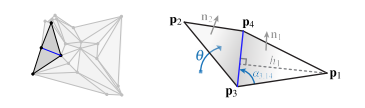
\includegraphics[width=0.5\linewidth]{hinge.png}
\caption{\label{fig:hinge}Dihedral crease constraint from Ghassei et al.}
\end{figure}
The constraint is rather simple: 
\[C = \theta - \theta_{goal}\]
We also want to know $\nabla C_i$, the gradient of $C$ at point $\textbf{x}_i$. We get: 
\[\nabla C = [\frac{\partial \theta}{\partial \textbf{x}_1},\frac{\partial \theta}{\partial \textbf{x}_2},\frac{\partial \theta}{\partial \textbf{x}_3},\frac{\partial \theta}{\partial \textbf{x}_4}]\]

Following the orientation given by Figure \ref{fig:hinge}, the derivatives for flap vertices $\textbf{x}_1, \textbf{x}_2$ are proportional to the normals of their respective triangles:
\[\frac{\partial \theta}{\partial \textbf{x}_1} = \frac{\textbf{n}_1}{h_1}, \frac{\partial \theta}{\partial \textbf{x}_2} = \frac{\textbf{n}_2}{h_2}\]
The derivatives for edge vertices $\textbf{x}_3, \textbf{x}_4$ are the weighted sum of the flap vertex derivatives. 
\[\frac{\partial \theta}{\partial \textbf{x}_3} = \frac{-\cot\alpha_{4, 31}}{\cot \alpha_{3,14}+\cot \alpha_{4,31}}\frac{\textbf{n}_1}{h_1} + \frac{-\cot\alpha_{4, 23}}{\cot \alpha_{3,42}+\cot \alpha_{4,23}}\frac{\textbf{n}_2}{h_2}\]
\[\frac{\partial \theta}{\partial \textbf{x}_4} = \frac{-\cot\alpha_{3, 14}}{\cot \alpha_{4,31}+\cot \alpha_{3,14}}\frac{\textbf{n}_1}{h_1} + \frac{-\cot\alpha_{3, 42}}{\cot \alpha_{4,23}+\cot \alpha_{3,42}}\frac{\textbf{n}_2}{h_2}\]

\section{Implementation Details}

We created a fabric simulation harness in Rust that is compiled to Web-Assembly (Wasm), and rendered using WebGPU. The harness can be run in-browser or as a headless binary for advanced debugging. We set up a simple user interface in the browser to adjust the parameters. The github repository can be found at https://github.com/txst54/wasm-cloth-sim. A browser-ready version is up at my website: https://cloth.clintwang.com. 

\subsection{Architecture}
The Rust core of the simulation is located in \verb|/rust|. All architecture-specific details (Wasm versus native binary) can be found in \verb|/rust/src/arch|. GPU-support is only enabled in the Wasm package, and the native binary is several commits behind the Wasm package, so outputs may not look the same. 

The Wasm package can be built using \verb|cd rust && wasm-pack build --target web --features gpu|. Since Wasm packages are compiled as a library, the "main" function of the Wasm package can be found in \verb|/rust/src/arch/wasm/harness.rs|. 

Since the native binary is compiled as a binary, the binary entry point can be found at \verb|/rust/bin/native.rs| and wraps \verb|/rust/src/arch/native/harness.rs|. 

If the GPU compute shaders in particle cloth or particle paper cause issues, the simulation can be reverted to the serial Gauss-Seidel CPU implementation by omitting the \verb|gpu| feature flag. All code relating to the user interface wrapping the Wasm package is located in \verb|/src|. 

\subsection{Available Simulations}

\begin{table}[H]
\centering
\begin{tabular}{l|r}
URL & Simulation \\\hline
\verb|/| & Triangle Mesh Cloth Simulation + Rotating BVH Rigid Body \\
\verb|/paper| & Triangle Mesh Paper Simulation \\
\verb|/particle_cloth| & GPU Particle Cloth Simulation + Static SDF Rigid Body \\
\verb|/particle_paper| & GPU Particle Paper Simulation
\end{tabular}
\caption{\label{tab:widgets}URLs for different simulations}
\end{table}
We offer 4 simulations located at different sub-URLs. The triangle mesh simulations run shape-matching PBD constraints by default while the particle cloth simulations only run distance XPBD constraints for cloth structure. We have a UI that allows the user to adjust several parameters relating to the simulation. Since scales for parameters $k_i \in [0, 1]$ may be very small, or on the exponential magnitude, we recommend manually entering numbers into inputs if the sliders do not prove sufficient. Damping and timestep are examples of this. 

\subsection{Available Crease Patterns}

\begin{table}[H]
\centering
\begin{tabular}{l|r}
Crease Pattern & Description \\\hline
\verb|line.cp| & A single vertical crease \\
\verb|lines.cp| & Two vertical creases \\
\verb|waterbomb.cp| & A traditional origami base \\
\verb|miura_ori.cp| & A classic and easy to fold origami tessellation \\
\verb|waterbomb_tess.cp| & A classic and harder to fold origami tessellation \\
\verb|yaccho.cp| & Modern origami "color-change" model. Designed and provided by Kei Morisue. \\
\verb|hex_torso.cp| & Modern origami "hex-pleat" model. Designed by Clint.
\end{tabular}
\caption{\label{tab:widgets} Available crease patterns for paper simulation}
\end{table}

Once you have build the necessary packages, you can run the web UI using \verb|npm install && npm run dev|. Attached below are reference outputs you can compare to:

\begin{figure}[H]
\centering
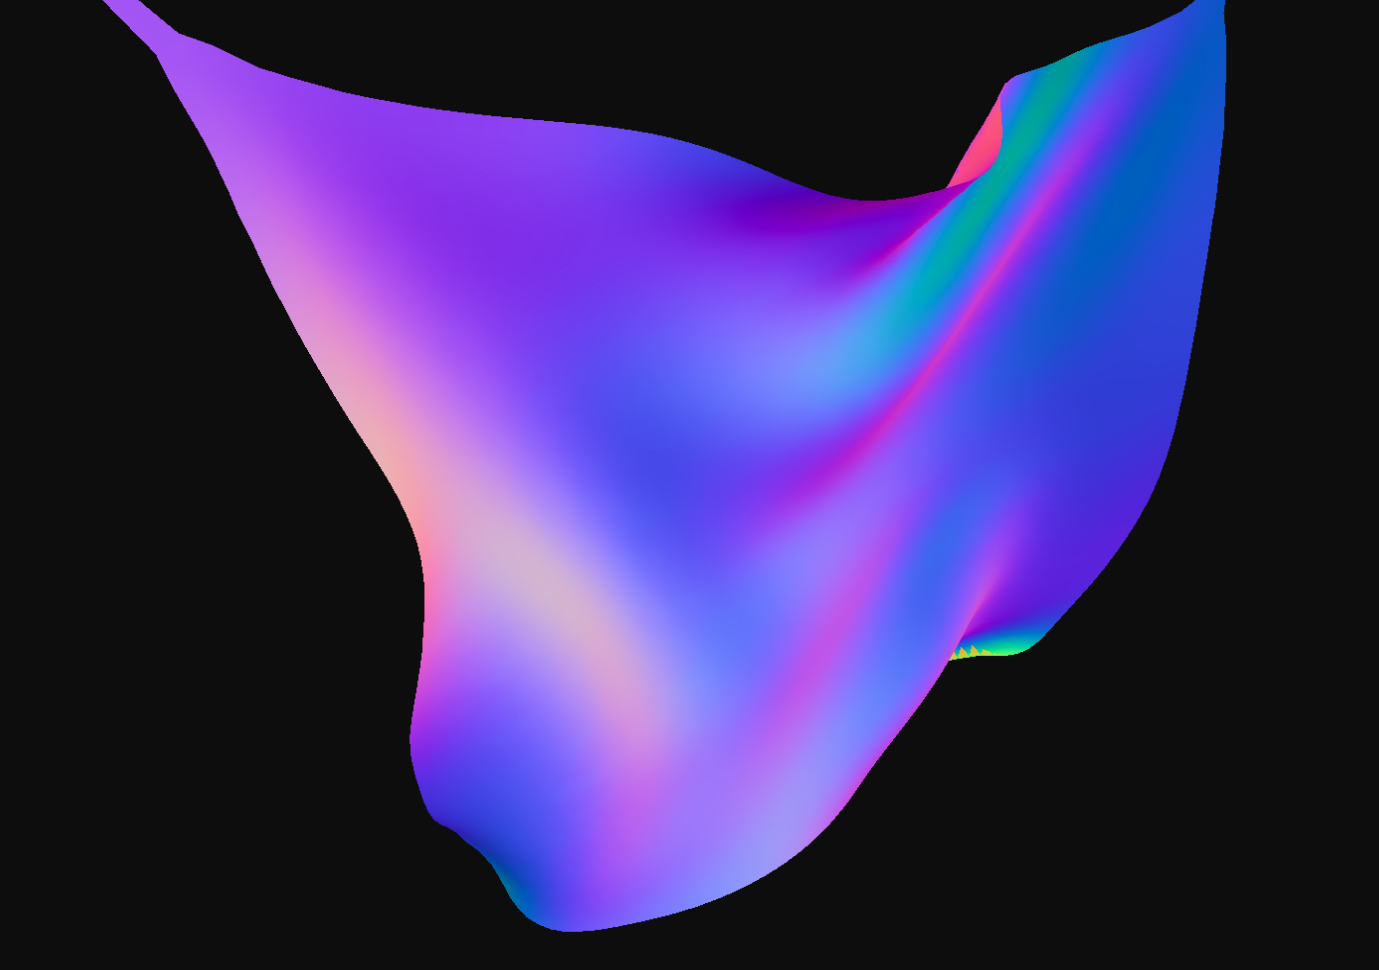
\includegraphics[width=0.4\linewidth]{triangle-cloth.png}
\caption{\label{fig:tc} Triangle mesh cloth simulation: PBD shape-matching cloth at resolution=64. }
\end{figure}

\begin{figure}[H]
\centering
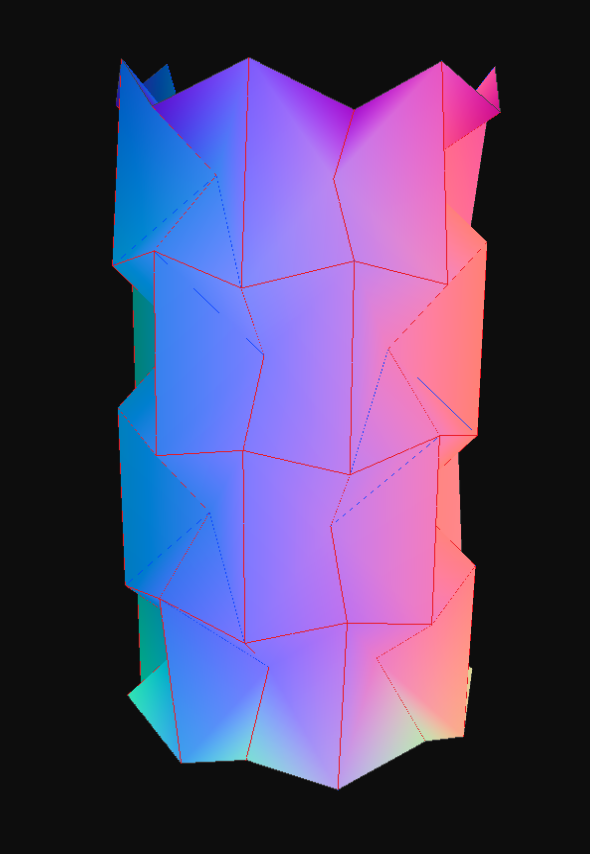
\includegraphics[width=0.4\linewidth]{triangle-paper-waterbomb.png}
\caption{\label{fig:tp} Triangle mesh paper simulation (XPBD shape-matching dihedral angle constraint): Waterbomb tessallation at resolution=1. }
\end{figure}

\begin{center}

% Row 3 ----------------------------------------------------
\begin{minipage}{0.45\linewidth}
    \centering
    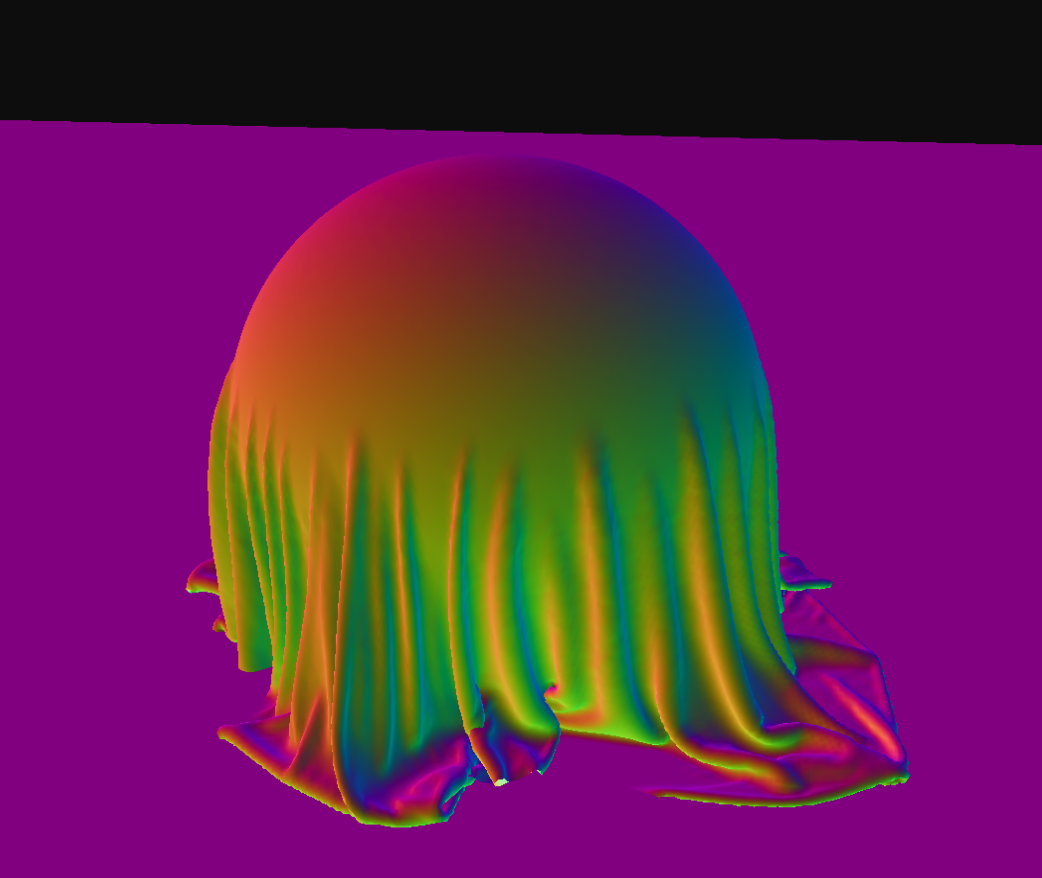
\includegraphics[width=\linewidth]{particle-cloth-lo-stp.png}
    \captionof{figure}{Particle cloth simulation (XPBD distance constraint): High-resolution cloth at 30 FPS, resolution=150, substeps = 1}
    \label{fig:pc-lo}
\end{minipage}
\hfill
\begin{minipage}{0.45\linewidth}
    \centering
    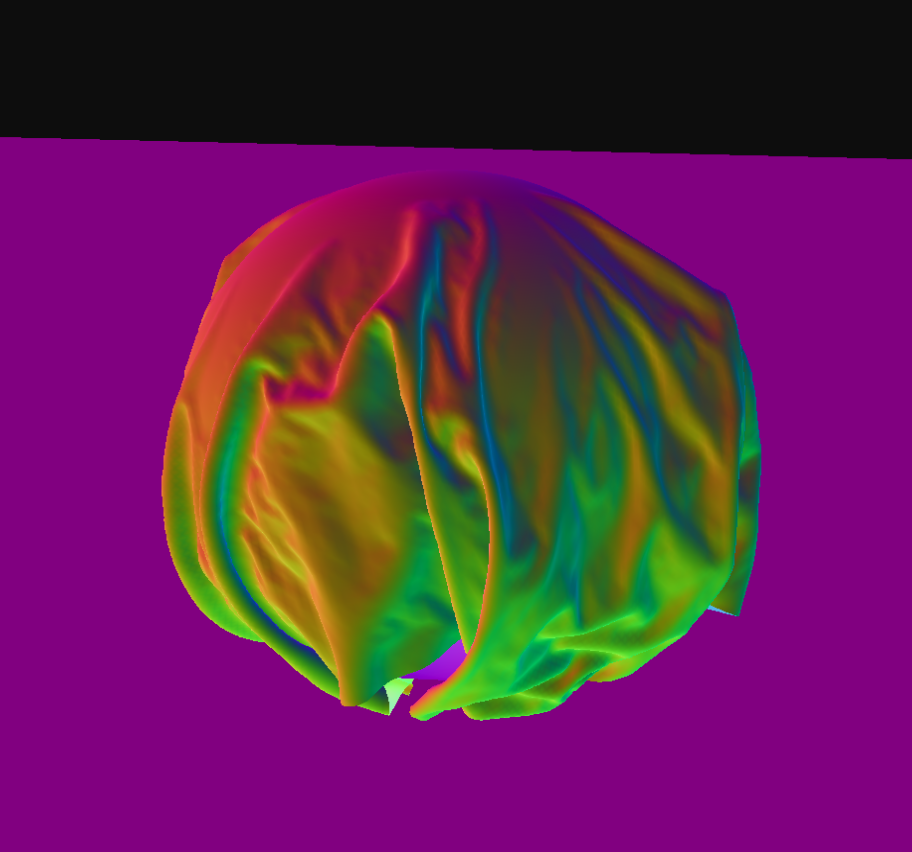
\includegraphics[width=\linewidth]{particle-cloth-hi-stp.png}
    \captionof{figure}{Particle cloth simulation (XPBD distance constraint): High-resolution cloth at 20 FPS, resolution=150, substeps = 10}
    \label{fig:pc-hi}
\end{minipage}

\end{center}

From Figures \ref{fig:pc-lo} and \ref{fig:pc-hi}, we see that using more substeps shows less stretching and higher material stiffness. 

\begin{figure}[H]
\centering
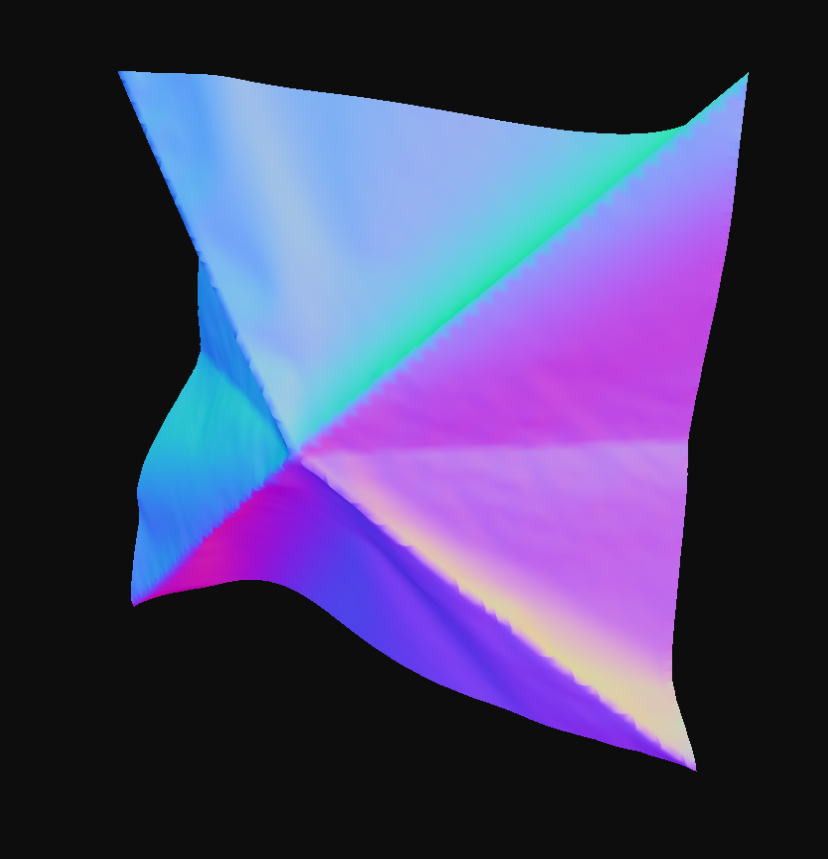
\includegraphics[width=0.5\linewidth]{particle-paper-waterbomb.png}
\caption{\label{fig:pp} Particle paper simulation (XPBD distance + dihedral angle constraint): Waterbomb base in a high resolution paper, resolution = 64. }
\end{figure}

One limitation of the particle XPBD paper simulation is that in high resolutions, the distance constraints become slightly unstable. Notice the small bumps in the paper in Figure \ref{fig:pp}. When we ran simulations in the triangle mesh PBD shape-matching paper simulation, the paper was smooth. This is because shape-matching provides high-fidelity projections onto the rest shapes. 

\bibliographystyle{alpha}
\bibliography{sample}

\end{document}